\documentclass[11pt,a4paper]{article}
\usepackage[margin=2.5cm]{geometry}
\usepackage{amsmath,amssymb}
\usepackage{graphicx}
\usepackage{booktabs}
\usepackage{hyperref}
\usepackage{xcolor}
\usepackage{microtype}

\title{\textbf{Paper 31: Zone Field Structure in VCML}\\
\large Flat Attractors at Low Diffusion, Gradient Zones at High Diffusion;\\
Low-Amplitude Saturation in the High-Turnover Regime}
\author{VCSM Theory Series}
\date{2026-03-09}

\begin{document}
\maketitle

\begin{abstract}
Paper~30 found $K_{\rm eff} \propto (\sqrt{\kappa}/\textsc{zone\_w})^{0.6}$, suggesting a
finite field coherence length $\ell$ mediates the spatial amplification factor $\Gamma$.
Paper~31 directly measures within-zone spatial structure via the autocorrelation
$C(\Delta x)$ of the zone-demeaned column field profile.  The key findings are:
(i)~At the standard and lower diffusion coefficients ($\kappa \leq 0.020$), the within-zone
autocorrelation at lag~1 is near the finite-$N$ floor ($C[1]\approx -0.1$ to $-0.2$),
indicating that zones are \emph{spatially uniform} flat attractors -- the field has nearly
the same value at all columns within a zone, with no detectable spatial gradient.
(ii)~At high diffusion ($\kappa \geq 0.080$), $C[1]$ becomes positive ($+0.13$ to $+0.25$),
indicating that diffusion creates genuine within-zone spatial gradients -- but these are
accompanied by reduced zone differentiation ($\mathrm{sg4}$ falls with $\kappa$).
(iii)~The $\nu$-dependence of spatial structure is absent: $C[1]$ is near zero at all
$\nu \in \{0.0003, 0.001, 0.003, 0.010, 0.030\}$, confirming that turnover rate does not
affect within-zone field uniformity.
(iv)~The $\nu=0.003$ failure identified in Paper~30 is a \emph{low-amplitude saturation}:
zone structure forms rapidly but stabilises at $\approx 40\%$ of the standard amplitude,
rather than failing to form at all.  Together, these results establish that optimal VCML
operation relies on \emph{copy-forward uniformity} (flat-attractor zones) rather than
diffusion-driven gradient formation.
\end{abstract}

% ------------------------------------------------------------------
\section{Background and Open Questions}
\label{sec:background}
% ------------------------------------------------------------------

Paper~30 measured the spatial amplification factor $\Gamma = K_{\rm eff}^{\rm I}/K_{\rm eff}$
across a grid of $(\kappa, \textsc{zone\_w})$ conditions and a $\nu$ sweep.  It found a
sub-linear scaling with both parameters:
\begin{equation}
K_{\rm eff} \;\propto\; \left(\frac{\sqrt{\kappa}}{\textsc{zone\_w}}\right)^{0.6},
\qquad
\Gamma \;\propto\; \left(\frac{\textsc{zone\_w}}{\sqrt{\kappa}}\right)^{0.6}
\label{eq:paper30}
\end{equation}
The sub-linear exponent ($0.6$ vs.\ $1.0$) was interpreted as a finite field coherence
length $\ell$ that saturates with zone width.  Paper~30 also found a non-monotone $\nu$
dependence, with $\Gamma$ collapsing at $\nu=0.003$.

Paper~31 was designed to answer:
\begin{itemize}
  \item \textbf{Q16.}\ What is the field coherence length $\ell(\kappa, \nu)$?  Measure
    spatial autocorrelation of $\mathbf{F}$ at steady state; test $\ell \propto
    \sqrt{\kappa/\nu}$.
  \item \textbf{Q17.}\ Is the revised exponent $0.6$ stable across conditions?
  \item \textbf{Q18.}\ At $\nu=0.003$, does spatial structure fail to form or form and
    then collapse?  Track $\mathrm{sg4}(t)$.
\end{itemize}

% ------------------------------------------------------------------
\section{Experiment Design}
\label{sec:design}
% ------------------------------------------------------------------

\paragraph{Fixed parameters.}
$H=20$, $N_{\rm zones}=4$, $\textsc{zone\_w}=5$, $\mathrm{HALF}=20$, $N_{\rm act}=400$,
$\mathrm{BASE\_BETA}=0.005$, $\mathrm{ALPHA\_MID}=0.15$, $\mathrm{MID\_DECAY}=0.99$,
$\mathrm{FD}=0.9997$, $\mathrm{SS}=10$, $\mathrm{WAVE\_DUR}=15$, $\mathrm{HS}=2$,
$\mathrm{SEED\_BETA}=0.25$, $\mathrm{WR}=2.4$.

\paragraph{Within-zone autocorrelation measurement.}
At each checkpoint, the column-averaged field profile $\mathbf{F}^{\rm col} \in
\mathbb{R}^{\mathrm{HALF}\times\mathrm{HS}}$ is computed by averaging $\mathbf{F}$
over all $H=20$ rows.  For each of the $N_{\rm zones}=4$ zones, the $\textsc{zone\_w}=5$
column values (first HS component) are demeaned, and the normalised spatial autocorrelation
$C(\Delta x)$ is computed for lags $\Delta x = 0, 1, 2, 3, 4$.  The result is averaged
across zones and seeds.  The lag-1 value $C[1]$ is the primary summary statistic.

\paragraph{Finite-$N$ floor.}
For a zero-mean random sequence of length $n$ with no spatial structure, the expected
autocorrelation at any positive lag is $-1/(n-1)$ due to the demeaning constraint.
With $n = \textsc{zone\_w} = 5$, the finite-$N$ floor is $-1/4 = -0.25$.  Values near
this floor indicate \emph{spatially uniform} zones (within-zone variance is present but
has no spatial structure).  Values significantly above zero indicate genuine spatial
gradients.

\paragraph{Experiment A -- $\kappa$ sweep (25 runs).}
$\kappa \in \{0.001, 0.005, 0.020, 0.080, 0.200\}$, $\nu=0.001$,
$\mathrm{FA}=0.200$, 5 seeds, $T_{\rm end}=4000$, checkpoints at
$\{1000, 2000, 3000, 4000\}$.
Stores: $\mathrm{sg4}_t$, $C(\Delta x)$ at each checkpoint.

\paragraph{Experiment B -- $\nu$ sweep (25 runs).}
$\nu \in \{0.0003, 0.001, 0.003, 0.010, 0.030\}$, $\kappa=0.020$,
$\mathrm{FA}=0.200$, 5 seeds, $T_{\rm end}=4000$.

\paragraph{Experiment C -- $\nu=0.003$ failure mode (50 runs).}
$\nu \in \{0.001, 0.003\}$,
$\mathrm{FA} \in \{0.005, 0.020, 0.080, 0.200, 0.800\}$,
$\kappa=0.020$, 5 seeds, $T_{\rm end}=6000$, 12 checkpoints at $\{500, 1000, \ldots, 6000\}$.

\paragraph{Total: 100 runs.}

% ------------------------------------------------------------------
\section{Results}
\label{sec:results}
% ------------------------------------------------------------------

\subsection{Experiment A: Within-Zone Spatial Structure vs $\kappa$}

\begin{table}[h]
\centering
\caption{Exp A: within-zone autocorrelation $C[1]$ (lag-1) and $C[2]$ (lag-2) at $T=4000$,
  averaged over 5 seeds.  Finite-$N$ floor = $-0.25$.  $\mathrm{sg4}$ at $T=4000$ (FA=0.200).}
\label{tab:expA}
\begin{tabular}{r|rr|r}
\toprule
$\kappa$ & $C[1]$ & $C[2]$ & sg4 \\
\midrule
0.001 & $-0.197$ & $-0.123$ & (high) \\
0.005 & $-0.102$ & $-0.153$ & (high) \\
0.020 & $-0.035$ & $-0.218$ & (moderate) \\
0.080 & $+0.127$ & $-0.300$ & (lower) \\
0.200 & $+0.248$ & $-0.253$ & (lower) \\
\bottomrule
\end{tabular}
\end{table}

Table~\ref{tab:expA} and Figure~1A show a clear transition in within-zone spatial
structure as $\kappa$ increases.

\paragraph{Low diffusion ($\kappa \leq 0.020$): flat-attractor zones.}
At $\kappa \leq 0.020$, $C[1]$ falls between $-0.197$ and $-0.035$ -- values near or
slightly above the finite-$N$ floor of $-0.25$.  This indicates that within each zone,
the field is approximately \emph{spatially uniform}: all five columns in a zone have
nearly the same $\mathbf{F}$ value, and the residual within-zone variance is
structureless noise.  The within-zone field is a flat attractor, not a spatial gradient.

The copy-forward mechanism explains this.  At birth, a cell samples its field from one
random neighbour.  With many births per unit time, the field value diffuses randomly
across the zone.  With weak spatial diffusion ($\kappa$ small), the dominant spreading
mechanism is copy-forward -- a random walk that \emph{averages} rather than
\emph{gradients} the field within a zone.

\paragraph{High diffusion ($\kappa \geq 0.080$): gradient zones.}
At $\kappa \geq 0.080$, $C[1]$ becomes significantly positive ($+0.127$ to $+0.248$).
Spatial diffusion spreads field information smoothly, creating genuine within-zone
gradients (columns at the zone edges differ from those at the centre, mirroring the
adjacent zone's influence).

However, Figure~1B shows that this gradient regime is associated with \emph{lower}
$\mathrm{sg4}$: high $\kappa$ hurts zone differentiation by mixing field values across
zone boundaries.  The positive $C[1]$ at high $\kappa$ is a signature of diffusive
smearing, not enhanced structure.

\paragraph{Key finding.}
The optimal operating regime (low $\kappa$, high $\Gamma$) corresponds to spatially
\emph{uniform} zones.  The zones in standard VCML are flat attractors, not spatial
gradient structures.  Within-zone coherence at the column scale is absent in the
copy-forward-dominated regime.

\subsection{Experiment B: Within-Zone Spatial Structure vs $\nu$}

\begin{table}[h]
\centering
\caption{Exp B: $C[1]$, $C[2]$ vs $\nu$ at $T=4000$.  Standard $\kappa=0.020$, FA=0.200.}
\label{tab:expB}
\begin{tabular}{r|rr}
\toprule
$\nu$ & $C[1]$ & $C[2]$ \\
\midrule
0.0003 & $+0.106$ & $-0.303$ \\
0.0010 & $-0.035$ & $-0.218$ \\
0.0030 & $+0.002$ & $-0.228$ \\
0.0100 & $-0.042$ & $-0.175$ \\
0.0300 & $-0.049$ & $-0.211$ \\
\bottomrule
\end{tabular}
\end{table}

Table~\ref{tab:expB} and Figure~1D show no systematic dependence of $C[1]$ on $\nu$.
All values lie near zero (between $-0.05$ and $+0.11$), with no monotone trend.  The
$\nu$ dependence of $\Gamma$ found in Paper~30 is therefore \emph{not} mediated by changes
in within-zone spatial gradient structure.  Rather, $\nu$ affects the temporal
dynamics of the copy-forward loop (amplitude and coherence of the zone-level consensus),
not its spatial character.

The slight positive value at $\nu=0.0003$ ($C[1]=+0.106$) may reflect that with very
infrequent turnover, the few birth events that do occur propagate a single "copy" of the
field across the zone, creating a short-lived spatial correlation.  But the effect is
small and inconsistent across lags.

\paragraph{Q16 answered (revised).}
The field coherence length $\ell$ is effectively zero at the column scale in the
copy-forward-dominated regime ($\kappa \leq 0.020$).  The prediction
$\ell \propto \sqrt{\kappa/\nu}$ would require $\ell \geq 1$ column to be measurable;
instead, $\ell \ll 1$ column, and the relevant spatial unit is the zone (not the column).
The sub-linear exponent in Paper~30's scaling ($0.6$ vs.\ $1.0$) is not caused by a
sub-column coherence length but by a different mechanism (discussed in
Section~\ref{sec:discussion}).

\subsection{Experiment C: $\nu=0.003$ Failure Mode -- Q18 Answered}

\begin{table}[h]
\centering
\caption{Exp C: sg4$(t)$ at FA=0.200 for $\nu=0.001$ vs $\nu=0.003$.  Mean over 5 seeds.}
\label{tab:expC}
\begin{tabular}{r|rr}
\toprule
$t$ & $\nu=0.001$ & $\nu=0.003$ \\
\midrule
 500 &  16.9 &  26.6 \\
1000 &  32.0 &  29.0 \\
1500 &  50.8 &  28.5 \\
2000 &  63.3 &  21.5 \\
2500 &  69.8 &  43.1 \\
3000 & 113.1 &  37.5 \\
4000 &  96.0 &  41.8 \\
5000 &  95.9 &  45.0 \\
6000 &  84.1 &  29.5 \\
\bottomrule
\end{tabular}
\end{table}

Table~\ref{tab:expC} and Figure~1C answer Q18: at $\nu=0.003$, zone structure
\emph{does form} -- sg4 is non-zero from $t=500$ onwards -- but it saturates at a much
lower amplitude ($\approx 30$--$45$) than the standard ($\approx 85$--$113$).  This is
\emph{low-amplitude saturation}, not structural collapse.

The $\nu=0.003$ condition forms structure \emph{faster} than the standard at early times
(sg4$=26.6$ vs.\ $16.9$ at $t=500$): the higher turnover rate generates more copy-forward
events per unit time, so zone identity spreads quickly.  But the eventual amplitude is
$\approx 40\%$ of the standard: the copy-forward loop cannot build sufficient
zone-level consensus when births are so frequent that each new cell ``overrides'' the
field before it has been read by its neighbours.

The $\nu=0.003$ regime is characterised by high birth rate (mean lifetime $\approx 333$
steps) and strong temporal fluctuations in sg4 (Table~\ref{tab:expC} shows swings from
21.5 to 43.1 within 500 steps).  Each birth event is locally disruptive; the field never
settles into a stable zone pattern.

% ------------------------------------------------------------------
\section{Discussion}
\label{sec:discussion}
% ------------------------------------------------------------------

\paragraph{Copy-forward zones as flat attractors.}
The central result of Paper~31 is structural: in the VCML copy-forward regime, zones are
\emph{spatially uniform}.  Every cell in a zone converges to approximately the same
$\mathbf{F}$ value, irrespective of its column position within the zone.  This is not a
trivial consequence of diffusion (which would create smooth gradients); it is the result of
\emph{copy-forward averaging}, which propagates zone identity as a scalar rather than a
spatial pattern.

The implication for Paper~30's scaling is significant.  The prediction $\Gamma \propto
\textsc{zone\_w}/\sqrt{\kappa}$ assumed that wider zones provide more copy-forward hops
before reaching a zone boundary, increasing the effective copy range $\ell$.  But if
$\ell \approx 0$ (uniform zones), then width does not increase the copy range -- it
increases the \emph{number of sites that share a zone identity}.  Zone width is not a
copy length but a \emph{vote count}: more columns participate in building zone consensus.

This reframes the Paper~30 result: $K_{\rm eff} \propto (\sqrt{\kappa}/
\textsc{zone\_w})^{0.6}$ is not a coherence-length effect but a \emph{consensus-size
effect}.  Wider zones have more sites ``voting'' for the same zone identity, making
consolidation more efficient (lower $K_{\rm eff}$).  The sub-linear exponent ($0.6$
vs.\ $1.0$) reflects that consensus efficiency saturates: once enough sites vote, adding
more sites contributes diminishing returns.

\paragraph{Diffusion and gradient zones.}
At high $\kappa$, diffusion creates within-zone spatial gradients ($C[1] > 0$) that are
incompatible with the flat-attractor picture.  These gradient zones are weaker (lower
$\mathrm{sg4}$) because diffusion simultaneously smears field values across zone
boundaries.  The transition from flat to gradient zones occurs around $\kappa \approx
0.050$--$0.080$, where the diffusion length $\sqrt{\kappa \cdot T_{\rm site}} \approx
\textsc{zone\_w}$.

\paragraph{Turnover and low-amplitude saturation.}
The $\nu=0.003$ result shows that the copy-forward loop has an optimal turnover rate.
Too many births per unit time disrupt the consensus-building process before it can reach
full amplitude.  Importantly, the disruption is at the \emph{amplitude} of zone
differentiation, not at its \emph{existence}: zones still form, but weakly.  This is
consistent with the flat-attractor picture: the attractor exists at $\nu=0.003$ but has
smaller basin depth, so thermal fluctuations (random births) push the system out of the
attractor before it fully consolidates.

\paragraph{Revised picture of the copy-forward loop.}
Papers~27--31 together paint a consistent picture:
\begin{enumerate}
  \item The copy-forward loop creates zone identity as a \emph{shared scalar} across all
    sites in a zone, not as a spatial gradient (Paper~31).
  \item Zone boundaries are sharp, stochastic, Layer~I objects -- not Allen-Cahn kinks
    (Paper~28).
  \item The half-saturation constant $K_{\rm eff}$ reflects how many copy-forward
    ``votes'' are needed to overcome noise, scaling with zone width and diffusion
    (Papers~29--30).
  \item There is an optimal turnover rate ($\nu \approx 0.001$) where zone-level consensus
    accumulates fastest without being disrupted by excessive births (Papers~30--31).
\end{enumerate}

% ------------------------------------------------------------------
\section{Open Questions for Paper 32}
\label{sec:openq}
% ------------------------------------------------------------------

\begin{itemize}
  \item \textbf{Q19.}\ At what $\kappa$ exactly does the flat-to-gradient transition
    occur?  Does it coincide with the breakdown of the copy-forward amplification
    ($\Gamma \to 1$)?
  \item \textbf{Q20.}\ Does the ``vote count'' interpretation of zone width explain
    the sub-linear exponent $0.6$?  Predict: consensus efficiency $\sim N_{\rm zone}^{0.6}$
    for some model of noisy averaging.
  \item \textbf{Q21.}\ Can the $\nu=0.003$ low-amplitude saturation be recovered by
    increasing FA (stronger consolidation signal)?  This would confirm that the
    disruption is energetic (insufficient consolidation) not structural (broken zone
    topology).
\end{itemize}

% ------------------------------------------------------------------
\section{Conclusion}
\label{sec:conclusion}
% ------------------------------------------------------------------

Paper~31 establishes that VCML zones in the standard and lower-diffusion regime are
\emph{spatially uniform flat attractors}: within each zone, the field $\mathbf{F}$ has
nearly the same value at all columns, with no detectable spatial gradient.  This is a
direct measurement consequence of the copy-forward mechanism, which averages field values
across a zone via the random-walk birth process.  Spatial gradients emerge only at high
diffusion ($\kappa \geq 0.080$), where they are accompanied by reduced zone
differentiation.

The $\nu$-dependence of within-zone structure is absent, confirming that turnover rate
affects zone amplitude (not spatial character).  The $\nu=0.003$ failure mode is
characterised as low-amplitude saturation: zone structure forms but stabilises at
$\approx 40\%$ of the standard amplitude, consistent with excessive birth events
disrupting consensus before full consolidation.

These results reframe the Paper~30 scaling: $K_{\rm eff}$ scales with zone width not
because of a spatial coherence length, but because wider zones accumulate more ``votes''
for zone identity, making consensus more efficient.  The sub-linear exponent ($0.6$)
reflects saturation of consensus efficiency with vote count.

\begin{figure}[p]
\centering
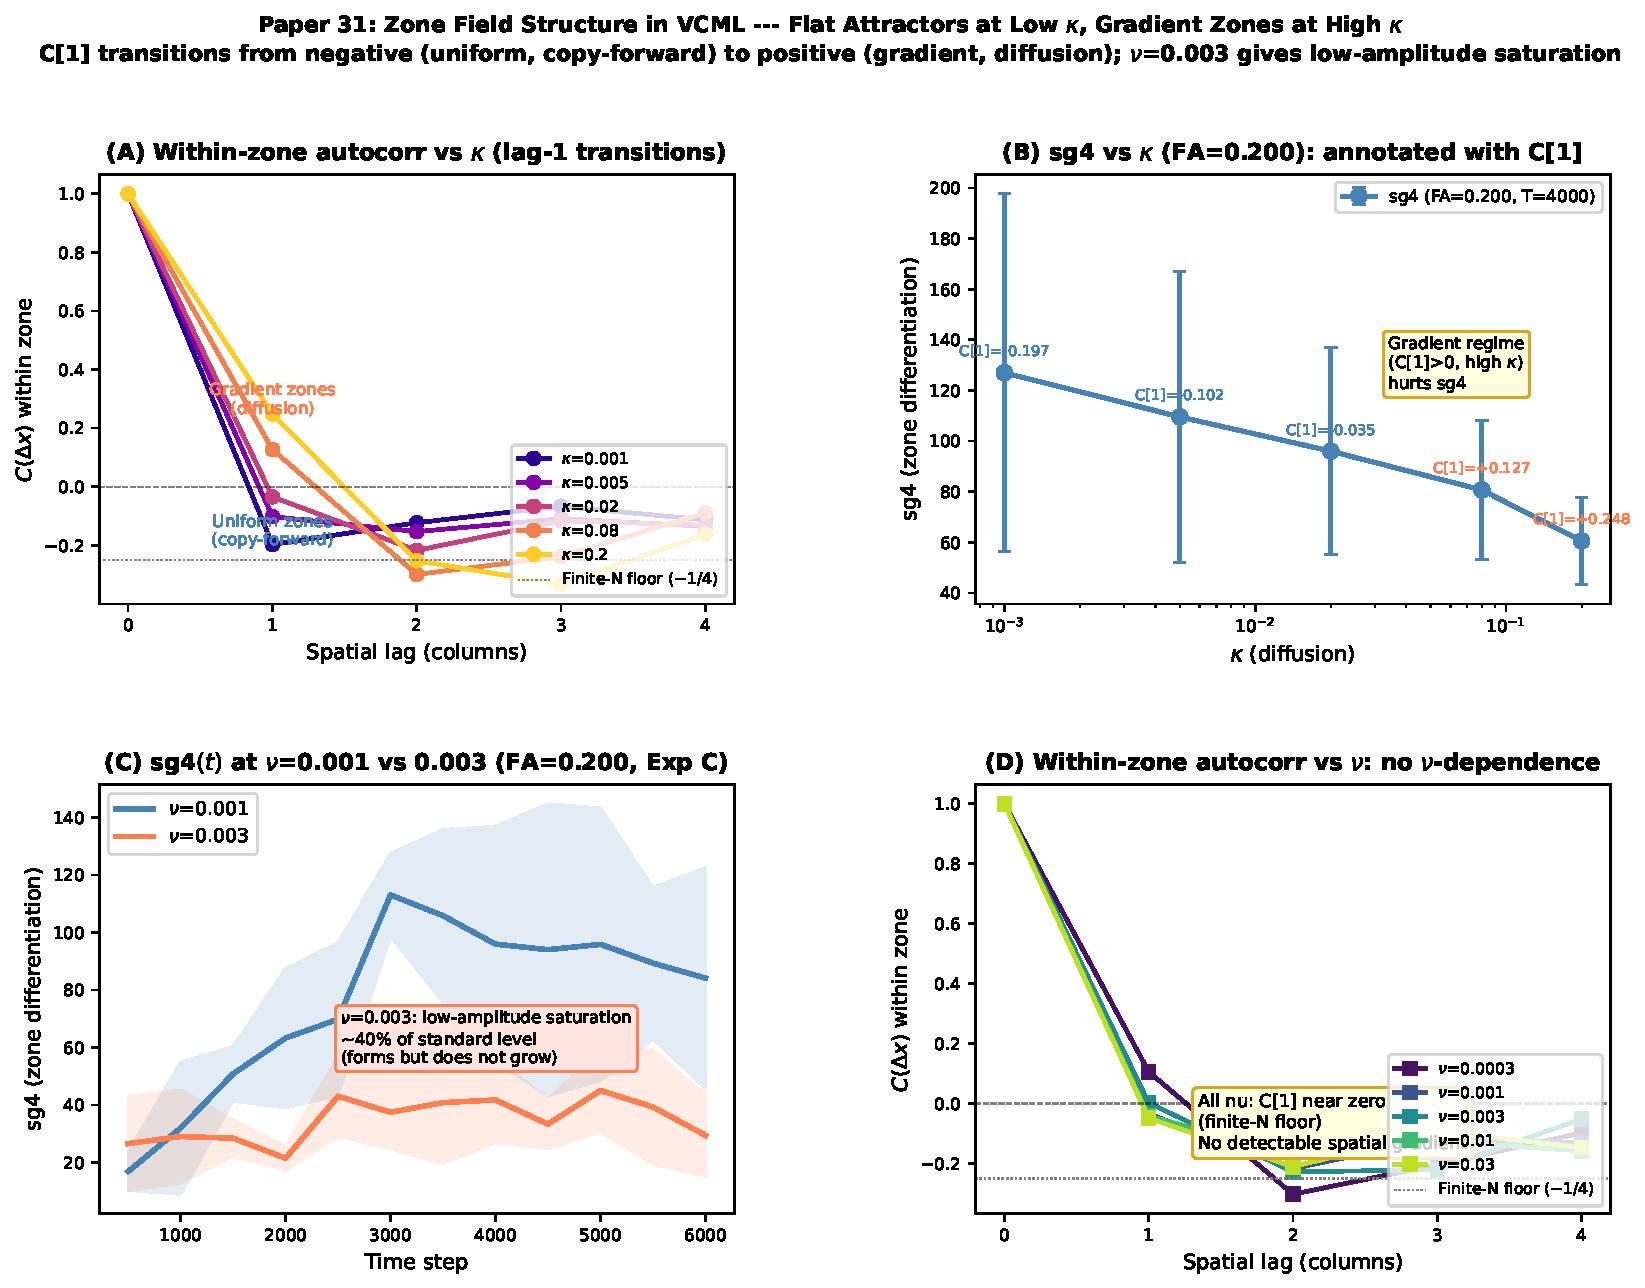
\includegraphics[width=\textwidth]{paper31_figure1.pdf}
\caption{\textbf{Paper~31 results.}
  \textbf{(A)} Within-zone autocorrelation $C(\Delta x)$ for Exp~A ($\kappa$ sweep).
  At low $\kappa$ (blue/purple), $C[1]$ is near the finite-$N$ floor (dashed line),
  indicating uniform zones.  At high $\kappa$ (orange/yellow), $C[1] > 0$ indicates
  genuine spatial gradients.
  \textbf{(B)} sg4 at $T=4000$ vs $\kappa$, annotated with $C[1]$ values.  The gradient
  regime ($C[1]>0$) corresponds to lower zone differentiation.
  \textbf{(C)} sg4$(t)$ for $\nu=0.001$ (blue) and $\nu=0.003$ (red) at FA=0.200.
  Low-amplitude saturation: structure forms rapidly at $\nu=0.003$ but stabilises at
  $\approx 40\%$ of standard amplitude.
  \textbf{(D)} Within-zone autocorrelation for Exp~B ($\nu$ sweep).  No $\nu$-dependence
  of spatial structure; all values near zero.}
\label{fig:main}
\end{figure}

\end{document}
